~\cite{WardellSelfForceReview}
\begin{equation}
  \Box\Psi^{ret}=-4\pi q\int\delta_4(x,z(\tau^\prime))d\tau^\prime
\end{equation}
In this equation, $\Box$ is the D'Alembertian and $z(\tau^\prime)$ is the evolving path of the source in spacetime as a function of the particle's proper time. The retarded field $\Psi^{ret}$, is defined to be the field determined by physics taking place at $t_r=t-\frac{|\vec{r}-\vec{r}^\prime|}{c}$; that is, at some distance away from the particle's path, the physical effects of gravity on the scalar field are retarded by light travel time. In the scalar approximation, the particle acts as a delta function point source, with a charge of $q$ and mass $m$. That charge may accelerate or evolve with time; see chapter~\ref{futurework}



\section{phi of t}
\subsection{Effective source}
\subsection{World tube}
\begin{figure}
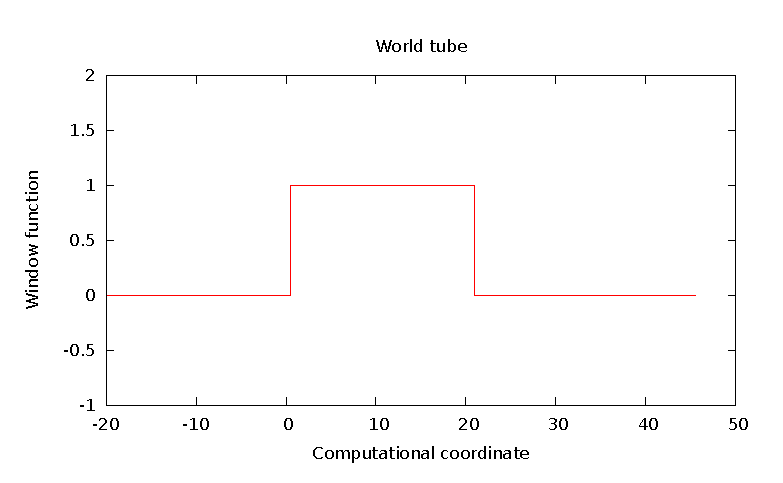
\includegraphics{worldTubeItself}
\caption{Spatial slice of the world tube window function.}
\end{figure}
\begin{figure}
  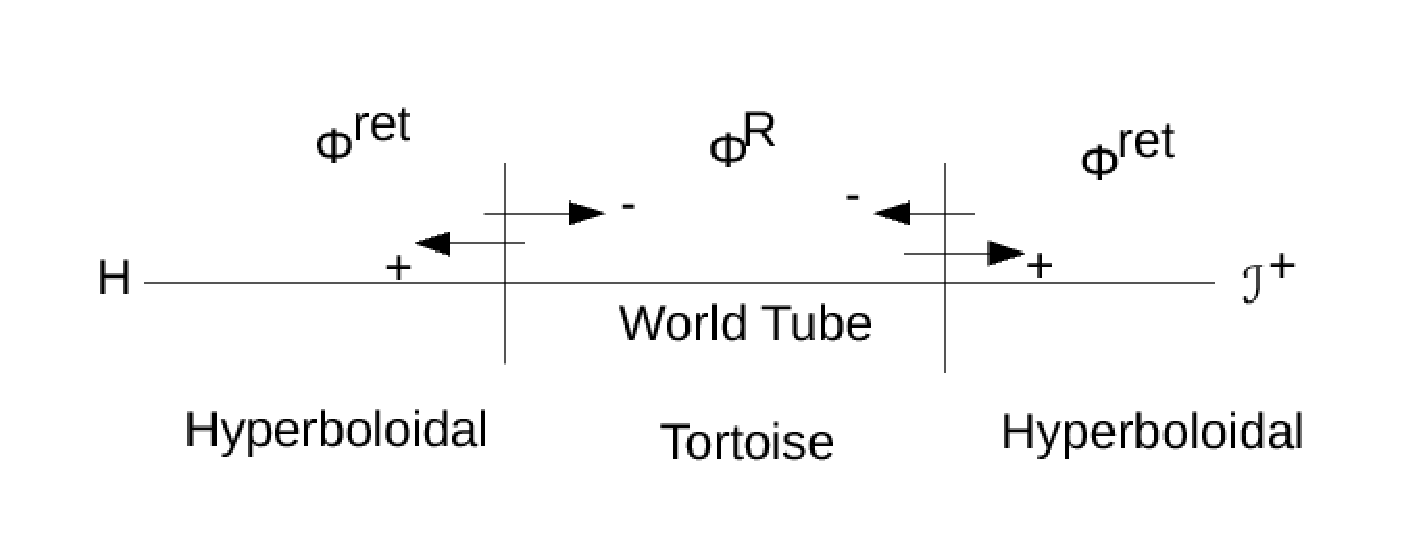
\includegraphics{WorldTube}
  \caption{Add or subtract the singular field to either side of the world tube boundary before performing the time dependent coordinate transform (or inverting it) to obtain the retarded field in the exterior region and the regularized field in the interior region.}

\end{figure}


\subsection{Comparison between C++ and Fortran codes}
\begin{figure}
  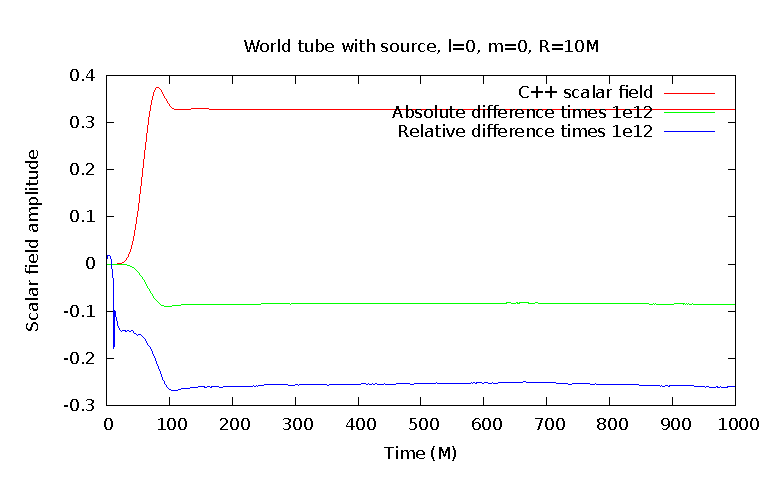
\includegraphics{wtcircl0m0}
  \caption{Comparison between Fortran and C++ codes for a particle on a circular orbit, l=0, m=0.}
\end{figure}
\begin{figure}
  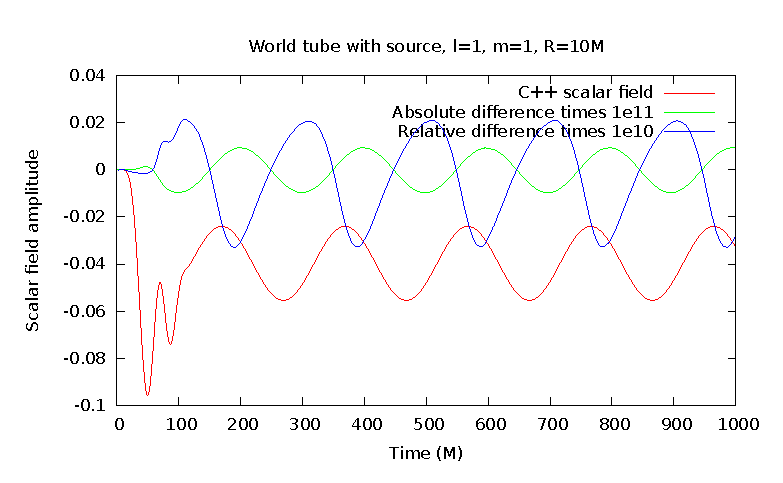
\includegraphics{wtcircl1m1}
  \caption{Comparison between Fortran and C++ codes for a particle on a circular orbit, l=1, m=1.}
\end{figure}
\begin{figure}
  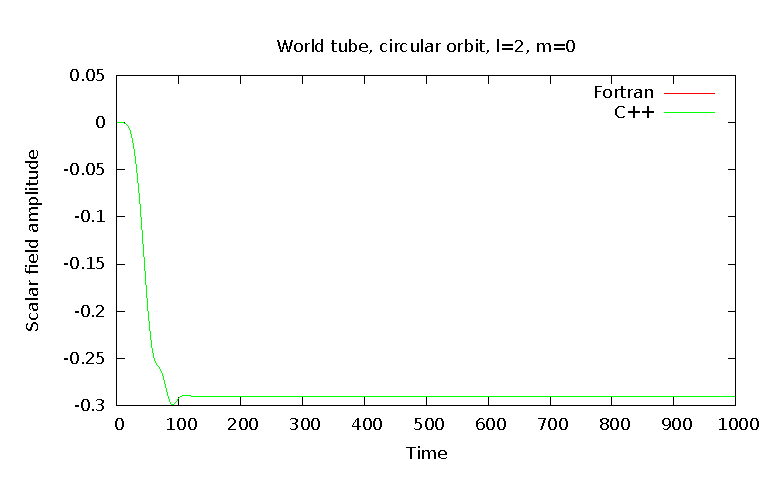
\includegraphics{wtcircl2m0}
  \caption{Comparison between Fortran and C++ codes for a particle on a circular orbit, l=2, m=0.}
\end{figure}
\begin{figure}
  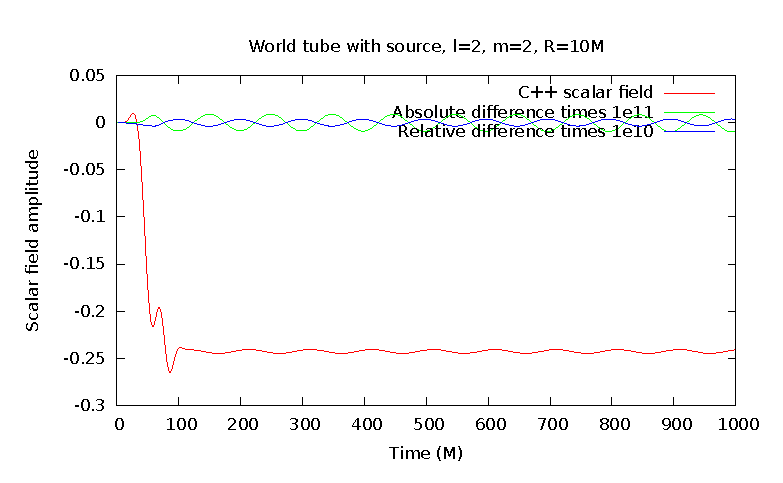
\includegraphics{wtcircl2m2}
  \caption{Comparison between Fortran and C++ codes for a particle on a circular orbit, l=2, m=2.}
\end{figure}
